% !TeX root = ../../main.tex

\chapter{Konzept}
In diesem Abschnitt wird kurz unser Konzept für die Umsetzung von Sfm erläutert. 
Insbesondere wird dabei erläutert, was in den einzelnen Schritten durchgeführt wird, und warum diese Schritte notwendig sind.
Details zur Implementierung werden in Kapitel~\ref{sec:implementation} beschrieben.

Das Konzept ist eine Kommandozeilen-Applikation, welche eine Pipeline mit Prozessen zur Rekonstruktion von Bildpunkten bereitstellt.
Die Pipeline ist in Abb.~\ref{fig:concept-pipeline} dargestellt.
Parameter, die für die einzelnen Prozesse benötigt werden, werden als Kommandozeilen-Argumente übergeben.
Der erste Prozess \emph{Kalibrierung} bestimmt die Parameter der Kamera, mit der die Bilder zur Rekonstruktion aufgenommen wurden.
Dieser Schritt ist nötig, da bei der Rekonstruktion die Kalibrierungsmatrix K benötigt wird.
Diese Matrix enthält Informationen über die Brennweite der Kamera und der Position des Hauptpunkts im Bild.
Des Weiteren wird bei der Kalibrierung auch die Verzerrungskoeffizienten der Linse der Kamera bestimmt. %TODO Koeffizienten in Kalibrierungskapitel erläutern
Damit kann die Verzerrung in den Bildern reduziert werden, was zu genaueren Ergebnissen beim Rekonstruieren führt.% TODO: muss belegt werden. gff im Kapitel Kalibrierung beschreiben 
Die Kalibrierung wird mit Hilfe eines Schachbrettmusters durchgeführt, weil *Insert befriedigende Begründug*.
Dementsprechend müssen zusätzliche Bilder für die Kalibrierung vom Nutzer bereitgestellt werden.
Das Kalibrieren der Kamera kann sehr zeitaufwendig sein.
Daher wird die Möglichkeit bereitgestellt, die Kameraparameter in einer Datei zu exportieren.
Diese Datei kann dann geladen werden, so dass eine weitere Kalibrierung mit dem Schachbrettmuster nicht mehr nötig ist. 
Es wird jedoch keine weiteren Features für die Verwaltung der Kalibrierungen angeboten.
Der Nutzer ist also selbst dafür verantwortlich zu wissen, welche Datei zu welcher Kamera gehört und welche Kalibrierungsdatei für die Pipeline benötigt wird. 

Der zweite Prozess umfasst das Feature Matching, welches benötigt wird, um korrespondierende Punkte in verschiedenen Bildern zu finden, die somit rekonstruiert werden können.
Wie in XXX beschrieben, wird hier in jedem Bild nach Keypoints gesucht und beschrieben.








\begin{figure}
    \centering
    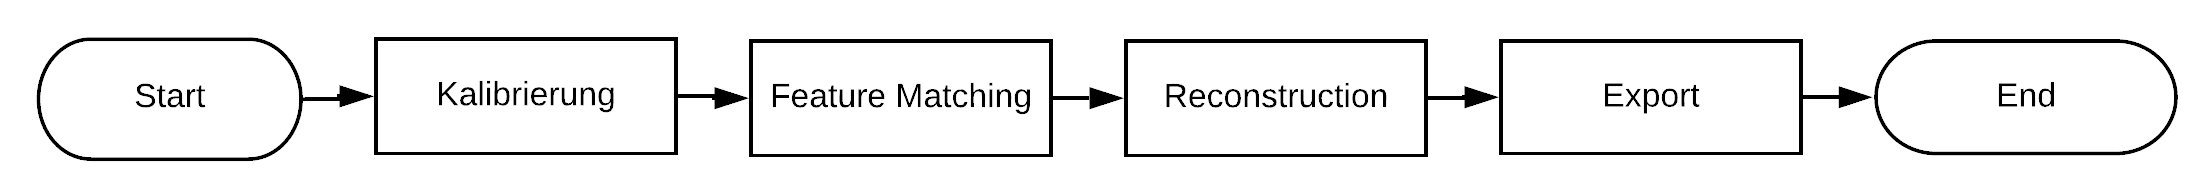
\includegraphics{src/img/konzept-pipeline-horizontal.png}
    \caption{Rekonstruktierungspipline des Konzepts}
    \label{fig:concept-pipeline}
\end{figure}
